\documentclass{article}
\usepackage{biblatex} %Imports biblatex package
\usepackage[utf8]{inputenc}
\usepackage{hyperref}
\usepackage{amsmath}
\usepackage{lipsum}
\usepackage{graphicx}
\usepackage{wrapfig}
\usepackage{float}
\usepackage{booktabs}
\usepackage[
backend=biber,
style=alphabetic,
]{biblatex}

\newcommand\numberthis[1][]{%
    \refstepcounter{equation}%
    \ifx#1\empty\else\label{eq:#1}\fi%
    \tag{\theequation}%
}
\newcommand{\mbf}[1]{\mathbf{#1}}
\newcommand{\be}{\begin{equation}}
\newcommand{\ee}{\end{equation}}
\newcommand{\mcl}[1]{\mathcal{#1}}


\title{Dataset generation for chiral metamaterials\vspace{-1em}}
\addbibresource{sample.bib} %Imports bibliography file
\author{(notes)}
\date{}

\begin{document}
\maketitle
\tableofcontents

\section{Unit cell based generation}


\subsection{Nassar-type unit cells.}

Nassar et al.\ \cite{nassar2018} design a lattice unit cell for elastic
cloaking that exhibits a rank-3 elasticity tensor \emph{lacking minor
symmetry}, as required by the Brun--Guenneau--Movchan (BGM) gauge of
transformation elasticity \cite{brun2009}.  The same unit-cell family is
directly relevant here because it provides a parametric, analytically
tractable class of \emph{chiral} (polar) lattices whose effective properties
can be sampled systematically.

\paragraph{Unit-cell architecture.}
A rectangular unit cell with aspect ratio $a/b$ contains:
\begin{itemize}
    \item two diagonal springs of stiffness $\alpha$, inclined at angle
          $\theta$ to the $\mathbf{n}$-direction;
    \item one vertical spring of stiffness $\beta$;
    \item a single rigid mass $m$ subjected to a restoring torque of
          stiffness $\kappa$ (torque per radian per unit cell area).
\end{itemize}
All contacts between the mass and the lattice frame are hinge-like, so the
cell supports no couple stresses from the springs alone.  The restoring torque
$\kappa$ is what makes the lattice \emph{polar}: it generates asymmetric
stress and breaks the minor symmetry of the effective elasticity tensor.

\paragraph{Effective constitutive law.}
In the normalised polar basis $(\mathbf{m},\mathbf{n})$, the homogenised
Hooke's law reads
\begin{equation}
\begin{bmatrix}
\sigma_{11} \\ \sigma_{22} \\ \sigma_{12} \\ \sigma_{21}
\end{bmatrix}
=
\begin{bmatrix}
\dfrac{ac^2\alpha}{b} & cs\alpha & 0 & 0 \\[6pt]
cs\alpha & \dfrac{b(as^2\alpha+2\beta)}{a} & 0 & 0 \\[6pt]
0 & 0 & \dfrac{b^2c^2\alpha\kappa}{\alpha(bc-as)^2+ab\kappa} &
          \dfrac{abcs\alpha\kappa}{\alpha(bc-as)^2+ab\kappa} \\[6pt]
0 & 0 & \dfrac{abcs\alpha\kappa}{\alpha(bc-as)^2+ab\kappa} &
          \dfrac{a^2s^2\alpha\kappa}{\alpha(bc-as)^2+ab\kappa}
\end{bmatrix}
\begin{bmatrix}
e_{11} \\ e_{22} \\ e_{12} \\ e_{21}
\end{bmatrix},
\label{eq:nassar-hooke}
\end{equation}
where $c=\cos\theta$, $s=\sin\theta$.  The off-diagonal shear block is
symmetric in the 12/21 sense (both off-diagonal entries equal), while the
normal block is symmetric; the tensor therefore has major symmetry
$C_{ijkl}=C_{klij}$ but lacks minor symmetry $C_{ijkl}\neq C_{jikl}$ in
general.


\paragraph{Inverse identification from an augmented Voigt matrix.}
Conversely, given an arbitrary augmented Voigt stiffness matrix $C_{IJ}$
(indices $I,J\in\{11,22,12,21\}$) that is block-diagonal and whose shear
block is rank-1, one can recover the five unit-cell parameters in closed form
by matching entries of \eqref{eq:nassar-hooke}.  

% Writing $r=a/b$,
% $c=\cos\theta$, $s=\sin\theta$, the normal block gives
% $C_{11,11} = rc^2\alpha$, $C_{11,22} = cs\alpha$,
% $C_{22,22} = (\alpha s^2+2\beta)/r$, and the shear block gives
% $C_{12,12} = c^2\alpha\kappa/\Delta$,
% $C_{12,21} = rcs\alpha\kappa/\Delta$,
% $C_{21,21} = r^2s^2\alpha\kappa/\Delta$
% with $\Delta = \alpha(c-rs)^2 + r\kappa$.
Eliminating the unknowns sequentially yields:
\begin{align}
    \theta &= \arctan\!\sqrt{\frac{C_{12,21}\,C_{11,22}}
                                   {C_{11,11}\,C_{12,12}}}\,,
    \label{eq:inv-theta}\\[4pt]
    \alpha &= \frac{C_{11,22}}{cs}\,,
    \label{eq:inv-alpha}\\[4pt]
    \frac{a}{b} &= \frac{s\,C_{11,11}}{c\,C_{11,22}}\,,
    \label{eq:inv-aspect}\\[4pt]
    \beta &= \frac{1}{2}\!\left(\frac{a}{b}\,C_{22,22}
             - \alpha s^2\right),
    \label{eq:inv-beta}\\[4pt]
    \kappa &= \frac{C_{12,12}\,\alpha\,(c-rs)^2}
                    {c^2\alpha - C_{12,12}\,r}\,.
    \label{eq:inv-kappa}
\end{align}
The rank-1 condition $C_{12,12}\,C_{21,21} = C_{12,21}^2$ serves as a
consistency check: it is satisfied identically for any stiffness produced by
\eqref{eq:nassar-hooke}.  When $c^2\alpha = C_{12,12}\,r$ the denominator
in \eqref{eq:inv-kappa} vanishes and $\kappa\to\infty$, corresponding to
the minor-symmetric limit $\lambda=\mu$.

\paragraph{Dataset generation strategy.}
A parametric dataset of Nassar-type unit cells can be generated by sampling the five parameters $(\lambda,\mu,f,\theta,\kappa)$, where $f$ is a normalised radial position in the cloak that controls the aspect ratio $a/b$ via \eqref{eq:inv-aspect}. 
The ground-truth labels can be computed either analytically from
\eqref{eq:nassar-hooke} or numerically via FE homogenisation.


\subsection{Cellular automaton based generation.}

Nakarmi et al.\ \cite{nakarmi2024} propose a data-driven framework for predicting the
non-linear stress--strain response of cellular structures under large uniaxial
compression.  The key novelty relevant to dataset generation is their use of
\emph{cellular automata} (CA) to generate a large and topologically diverse
library of unit cells.

\paragraph{Grid and initial state.}
Each unit cell is discretised on a $25\times25$ pixel grid (physical size
$2.5\,\text{mm}\times2.5\,\text{mm}$).  Each pixel takes a binary value: 1
(solid material, \emph{live}) or 0 (void, \emph{dead}).  The initial
population of live pixels is approximately 49\% ($\approx306$ out of 625).

\paragraph{Evolution rules.}
The topology evolves according to the following rules, applied simultaneously
to all interior pixels at every iteration:
\begin{enumerate}
    \item \emph{Border enforcement:} border pixels are permanently set to live,
          except for a random subset of adjacent \emph{gate} pixels that are
          set to dead, ensuring boundary connectivity while allowing some
          porosity.
    \item \emph{Birth:} a dead pixel becomes live if it has 5--8 live
          neighbours.
    \item \emph{Death:} a live pixel becomes dead if it has 0--3 live
          neighbours.
    \item \emph{Survival:} a pixel retains its current value if it has exactly
          4 live neighbours.
\end{enumerate}
Iteration continues until convergence (typically 7 steps with no further
change).

\paragraph{Post-processing for connectivity.}
The converged CA map is inverted to yield a \emph{reverse map} (the solid
phase).  A flood-fill algorithm identifies all disconnected solid regions
$\mathcal{R}$.  A connection graph $G(u,v,m,n,r)$ is then built, where $u,
v\in\mathcal{R}$ are pairs of regions, $m,n$ are the nearest cells between
them, and $r$ is the minimum distance.  Kruskal's minimum spanning tree
algorithm on $G$ produces a spanning graph $K$ that links every disconnected
region with minimum total bridge length; bridges are drawn as 4-pixel-wide
connections.  Finally, in the original paper, the structure is mirrored along the vertical and
horizontal axes to produce a periodic unit cell.

\paragraph{Chiral assembly.}
The original CA procedure produces unit cells that are symmetric under reflection.
To introduce chirality, we can assemble four rotated copies of a single $25\times25$ CA tile — at $0°$,
$90$°, $180$°, and $270$° — into a single $50\times50$ unit cell
(Figure~\ref{fig:tile3_ca_chiral}).
Gate pixels are centred on each tile edge so that, after rotation, opposing gates remain
aligned and the assembled cell stays connected across the internal seams.
Figure~\ref{fig:ca_chiral_progression} shows successive stages of this process from
a freshly evolved CA map through to the final chiral $50\times50$ cell.

\begin{figure}[H]
    \centering
    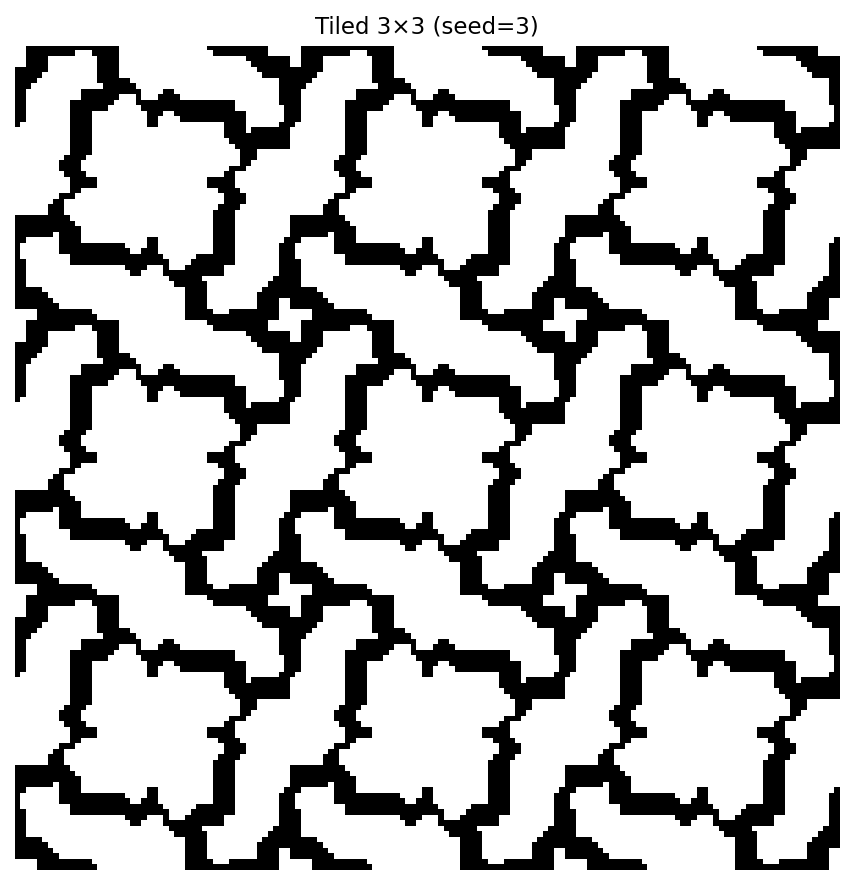
\includegraphics[width=0.45\textwidth]{../figures/tile3_ca_chiral.png}
    \caption{A single CA tile 3x3 obtained by assembling unit cells.}
    \label{fig:tile3_ca_chiral}
\end{figure}

\begin{figure}[H]
    \centering
    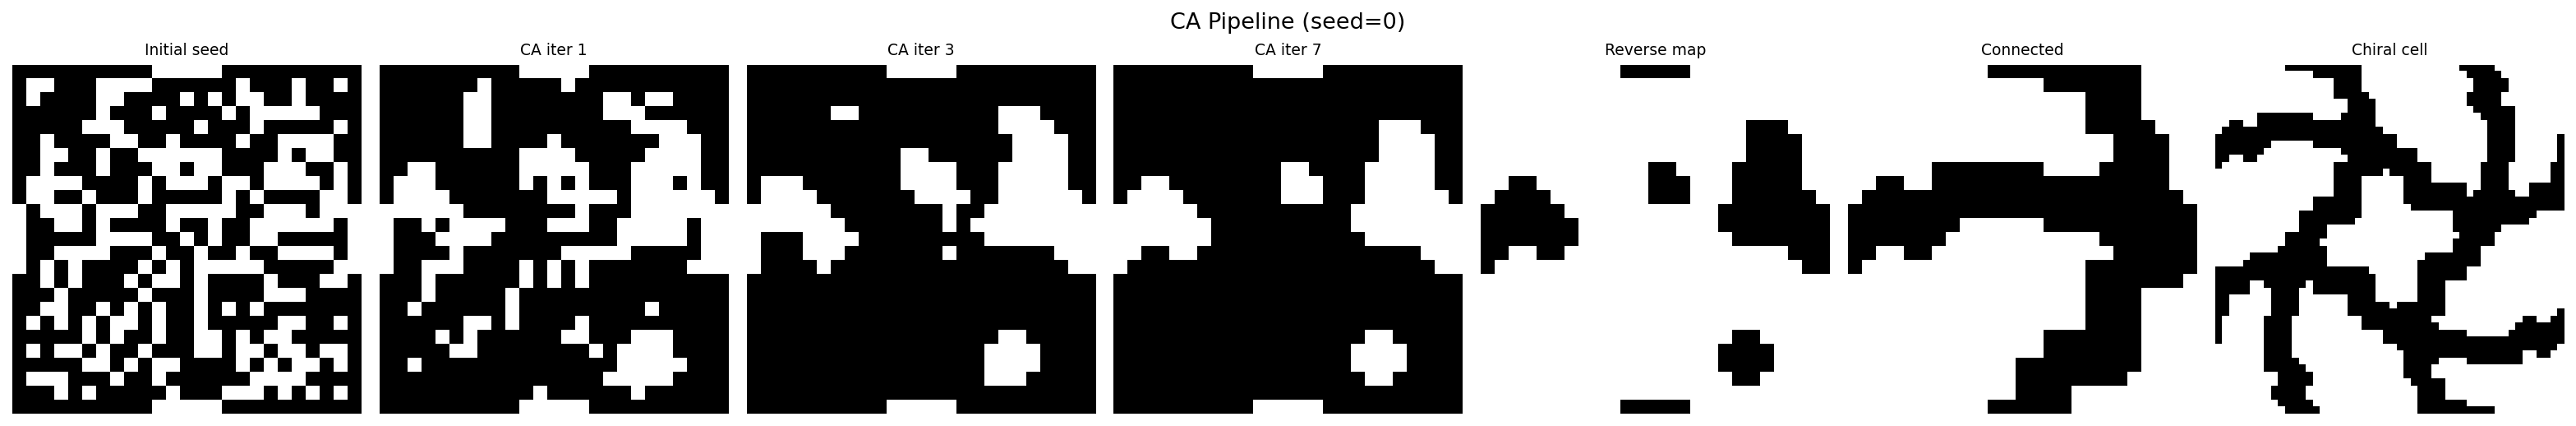
\includegraphics[width=0.85\textwidth]{../figures/ca_chiral_progression.png}
    \caption{Progression from random initialization to final chiral unit cell across the stages.}
    \label{fig:ca_chiral_progression}
\end{figure}

\paragraph{Squared (D2) assembly.}
For bulk dataset generation we also use a non-chiral variant in which the four
copies of the $25\times25$ CA tile are \emph{mirrored} rather than rotated (the
\texttt{squared} mode of \texttt{dataset/cellular\_chiral/bulk\_generate.py}, run
as \texttt{python -m dataset.cellular\_chiral.bulk\_generate --assembly squared}).
The top-left quadrant is copied directly, the top-right is reflected left--right,
the bottom-left up--down, and the bottom-right across both axes, so the assembled
$50\times50$ cell is invariant under reflection about both the horizontal and
vertical centre lines: it possesses $D_2$ (orthotropic) symmetry. Each cell is
generated with its live fraction drawn uniformly in $[0.20, 0.80]$, and the whole
library is written contiguously to a single memmapped array. The $D_2$ mirror
symmetry forces the effective stiffness to be orthotropic in the cell axes: the
normal--shear coupling components vanish ($C_{1112}=C_{2212}=0$) and minor
symmetry is retained, so the Cosserat shear asymmetry of
\eqref{eq:nassar-hooke} disappears ($C_{1212}=C_{2121}$, hence the chirality
index $\chi=0$). The tensor is then fully described by only four independent
components
\begin{equation}
  (C_{1111},\,C_{2222},\,C_{1212},\,C_{1122}),
  \label{eq:flat4}
\end{equation}
which is exactly the \emph{flat4} parametrisation implemented by
\texttt{C\_to\_flatC}/\texttt{flatC\_to\_C} in
\texttt{rayleigh\_cloak/materials.py}. This compact 4-vector (together with the
density $\rho$) is the per-cell label stored for the squared dataset and the
feature space over which the dataset GMM is fitted. The chiral cells of the
previous paragraph break minor symmetry and instead require the 6- or
10-parameter Cosserat representations; the flat4 form is appropriate precisely
because the squared cells are minor-symmetric.


% \subsection{Graph based representation (idea)}

% Unit cell topologies can be represented as planar graphs, where nodes
% correspond to distinct material vertices (or mass positions) and edges
% correspond to structural connections (beams, springs, or bonds) between them.
% This representation seems natural for lattice materials, so it is possible 
% to come up with a strategy for generating such graphs and lattices from graphs.

% \paragraph{Generative rules.}
% A dataset can be generated by defining:
% \begin{itemize}
%     \item \emph{Node types} $\mathcal{N}$ (e.g.\ block).
%     \item \emph{Edge types} $\mathcal{E}$ (e.g.\ axial spring, beam, torsion
%           spring).
%     \item \emph{Sampling rules} that draw random planar graphs consistent with
%           these constraints.
% \end{itemize}

% The 2D lattice geometry can be then rendered deterministically from the graph by
% assigning geometric parameters (thickness, length, curvature) that may be
% sampled independently, yielding a two-level generative model: topology (graph)
% $\to$ geometry (continuous parameters) $\to$ effective properties.

\section{Metrics of goodness of generated dataset}

\paragraph{Diversity.}
Diversity measures how spread out the dataset is in feature space.  
% Common metrics include:
% \begin{itemize}
%     \item Average pairwise distance in the effective-property space
%           $\langle d(C^{(i)}, C^{(j)})\rangle_{i\neq j}$.
%     \item Entropy of a kernel density estimate of the sample distribution.
%     \item The determinant $\det(\Sigma)$ of the sample covariance matrix
%           (volume of the occupied region in feature space).
% \end{itemize}
In the Nakarmi et al.\ framework \cite{nakarmi2024}, diversity of the
stress--strain curves is assessed via the explained variance captured by
the first few PCA components: a dataset in which 99.89\% of variance is
captured by 20 components is well-concentrated along those principal
directions.

\paragraph{Coverage.}
Coverage measures how well the dataset fills the target design space — i.e.\
whether all practically relevant property combinations are represented.  It can
be quantified as the fraction of a reference grid in property space that
contains at least one sample within a radius $\varepsilon$, or via the
Hausdorff distance between the sample set and the target region.

\paragraph{Chirality.}
For metamaterial cloaking applications, the dataset must contain a sufficient
fraction of chiral unit cells (those with broken minor symmetry).  Chirality
can be measured by the asymmetry index $\chi$ defined above:

\begin{equation}
    \chi = \frac{|C_{1212} - C_{2121}|}{C_{1212} + C_{2121}},
\end{equation}




% \section{Feasibility considerations}

% Before investing in a full dataset-generation and training pipeline, it is
% worth asking whether Nassar-type unit cells are at all realisable in a
% concrete (beton) substrate.  This section identifies the principal obstacles
% and catalogues techniques that could, in principle, overcome them.  The
% question of whether to incorporate these constraints into the dataset at this
% stage or simply leave them as a discussion point is addressed at the end.

% \paragraph{Baseline concrete parameters.}
% Standard structural concrete has approximately:
% \begin{align}
%     E   &\approx 25\text{--}35\,\text{GPa},
%     &\nu &\approx 0.18\text{--}0.22,
%     &\rho &\approx 2200\text{--}2400\,\text{kg\,m}^{-3}.
% \end{align}
% Taking representative values $E=30\,\text{GPa}$, $\nu=0.20$, these translate
% to Lam\'e parameters
% \begin{align}
%     \lambda &= \frac{E\nu}{(1+\nu)(1-2\nu)}
%              \approx 8.3\,\text{GPa},
%     &
%     \mu &= \frac{E}{2(1+\nu)}
%         \approx 12.5\,\text{GPa},
% \end{align}
% so that $\mu > \lambda$ for plain concrete.

% \paragraph{Realising hinge-like connections in concrete.}
% The Nassar lattice requires all connections between the central mass and the
% lattice frame to be \emph{hinge-like}: they must transmit force but impose no
% moment.  Concrete is a monolithic, brittle material with high moment stiffness
% at joints.  True hinges are therefore difficult to achieve without deliberate
% intervention.

% \paragraph{Possible mitigation strategies.}
% Several techniques could individually or jointly address the two problems
% above:

% \begin{itemize}

%     \item \textbf{Flexural ligaments (bending concrete strips).}
%           Thin concrete elements — notched sections or deliberately
%           slender connecting strips — deform primarily in bending and
%           therefore exhibit a low effective rotational stiffness relative
%           to their axial stiffness.  This approximates a hinge for
%           wavelengths much longer than the strip length.  

%     \item \textbf{Soft interlayers (elastomeric pads or polymer gaskets).}
%           Inserting elastomer or soft polymer layers at each
%           mass-to-frame contact provides a material with $\nu\approx0.5$
%           and $E\approx1$--$10\,\text{MPa}$ at the joint. 

%     \item \textbf{Embedded steel pins or bolts.}
%           Discrete steel dowels or pin-ended bolts connecting prefabricated
%           concrete blocks provide genuine load-path hinges with negligible
%           moment transfer.  The mass element would be a prefabricated
%           concrete or steel block; the frame elements would be slender
%           concrete ribs or steel rods; all joints would terminate in
%           standard pin connections.  This is the most direct mechanical
%           analogue of the Nassar unit cell, though it requires composite
%           construction and more careful FEM analysis.

%     \item \textbf{Fiber-reinforced or high-performance concrete.}
%           UHPC (ultra-high-performance concrete) and FRC (fiber-reinforced
%           concrete) can reach $\nu\approx0.25$--$0.28$, approaching or
%           satisfying the $\nu\geq\tfrac{1}{4}$ stability threshold.

% \end{itemize}

% \paragraph{Should this be addressed at the dataset-generation stage?}
% Two positions are defensible:
% \begin{enumerate}
%     \item \emph{Ignore for now and flag for discussion.}  The dataset is
%           generated over the full physically admissible parameter space
%           ($\lambda,\mu>0$, no sign constraint).  Samples with
%           $\mu>\lambda$ are labelled as ``concrete-infeasible'' but
%           retained in the training set.  This keeps the dataset general
%           and avoids baking in assumptions about the fabrication route
%           that may change.
%     \item \emph{Restrict to $\nu\geq1/4$ from the outset.}  Sampling only
%           from the $\lambda\geq\mu$ half-space guarantees that every
%           generated unit cell has a physically realisable (positive)
%           torsion spring constant, and the surrogate model never needs to
%           generalise outside the feasible regime.  The cost is a reduction
%           in dataset diversity.
% \end{enumerate}




\printbibliography


\end{document}
